\documentclass[11pt,a4paper]{article}
\usepackage[T1]{fontenc}\usepackage{lmodern}
\usepackage[margin=22mm,headheight=14pt]{geometry}
\usepackage{amsmath,amssymb,bm,booktabs,tabularx,array,graphicx,float,fancyhdr,microtype,xcolor}
\usepackage[colorlinks=true,linkcolor=blue!45!black,urlcolor=blue!45!black,citecolor=blue!45!black]{hyperref}
\setlength{\parindent}{0pt}\setlength{\parskip}{5pt}\renewcommand{\arraystretch}{1.15}
\pagestyle{fancy}\fancyhf{}\fancyhead[L]{\small QFT Project B | Step 2}\fancyhead[R]{\small Group B}\fancyfoot[C]{\thepage}
\newcommand{\dd}{\mathrm{d}}
\begin{document}\hypersetup{pageanchor=false}
\begin{titlepage}\centering\vspace*{3mm}

\includegraphics[width=36mm]{assets/bits_logo.png}\par\vspace{13mm}
{\Large\bfseries BITS PILANI K.K. BIRLA GOA CAMPUS\par}\vspace{3mm}
{\large\bfseries Department of Physics\par}\vspace{18mm}
{\LARGE\bfseries What Quantum Trace Can\\[2mm] a Heavy Particle Leave?\par}\vspace{6mm}
{\large Curvature--Spectator Entanglement\\and the Cosmological Collider\par}\vspace{10mm}
{\large\bfseries Step 2: Two-Oscillator Entropy\par}\vspace{17mm}
{\Large\bfseries Group-B\par}\vspace{5mm}
\begin{tabular}{ll}Priyansh Rawat & 2023B5A70968G\\Mayank Sinha & 2023B5A70942G\\Samarth Bhatnagar & 2023B5A70853G\end{tabular}
\vfill{\large Under Professor: Rudranil Basu\par}\vspace{7mm}{29 October 2026\par}
\end{titlepage}\setcounter{page}{1}\hypersetup{pageanchor=true}
\section{Normal modes and the reduced state}
We first test the entropy calculation on two coupled oscillators, where the ground state can be found exactly. In units $\hbar=1$,
\begin{equation}H=\frac{p_1^2+p_2^2}{2}+\frac12\bm{x}^{T}K\bm{x},\qquad K=\begin{pmatrix}1&c\\c&2\end{pmatrix}.\end{equation}
The eigenvalues are $(3\pm\sqrt{1+4c^2})/2$. Both are positive when $|c|<\sqrt2$, including the required $c=0.3$ and $0.6$ cases. If $K=U\,\mathrm{diag}(\omega_j^2)U^T$, the change of variables $\bm{y}=U^T\bm{x}$ and $\bm{p}_y=U^T\bm{p}$ gives independent normal modes. Their ground-state variances are $1/(2\omega_j)$ and $\omega_j/2$. Transforming back gives
\begin{equation}X=\langle\bm{x}\bm{x}^T\rangle=\tfrac12K^{-1/2},\qquad P=\langle\bm{p}\bm{p}^T\rangle=\tfrac12K^{1/2},\qquad\tfrac12\langle\{x_i,p_j\}\rangle=0.\end{equation}
Tracing out oscillator 2 retains $V_1=\mathrm{diag}(X_{11},P_{11})$. Its symplectic eigenvalue and entropy are
\begin{equation}\nu=\sqrt{\det V_1},\qquad s(\nu)=(\nu+\tfrac12)\ln(\nu+\tfrac12)-(\nu-\tfrac12)\ln(\nu-\tfrac12).\end{equation}
The convention $0\ln0=0$ gives zero entropy at $\nu=1/2$. At nonzero coupling, the normal modes involve both original oscillators. The joint ground state remains pure, while the reduced oscillator can be mixed. Entropy is measured in nats.
\begin{center}\small\begin{tabular}{lll}\toprule Coupling $c$ & $
u$ & Entropy (nats)\\\midrule
$0$ & $0.5$ & $0$\\
$0.3$ & $0.502816542$ & $0.0193599304$\\
$0.6$ & $0.512481339$ & $0.0672711138$\\\bottomrule\end{tabular}\end{center}
\newpage
\section{Numerical checks and interpretation}
The diagonalisation reproduces $\nu=0.5028165419863$ and $s=0.0193599304236$ at $c=0.3$. At $c=0$ the entropy vanishes. At $c=0.6$ it increases to $0.06727$.
A separate check uses the ground-state Gaussian wavefunction kernel $A=K^{1/2}$. Direct Gaussian integration gives
\begin{equation}\mathrm{Tr}\rho_1^2=\sqrt{\frac{\det A}{A_{11}A_{22}}}=\frac{1}{2\nu},\end{equation}
which agrees with the covariance result. A local rescaling $x_1\mapsto b x_1$, $p_1\mapsto p_1/b$ changes the individual variances but leaves their product and $s$ unchanged. The largest determinant change over $b=0.1,0.5,1,2,10$ is $5.551\times10^{-17}$. Thus squeezing a decoupled oscillator does not create inter-oscillator entanglement.
\begin{figure}[H]\centering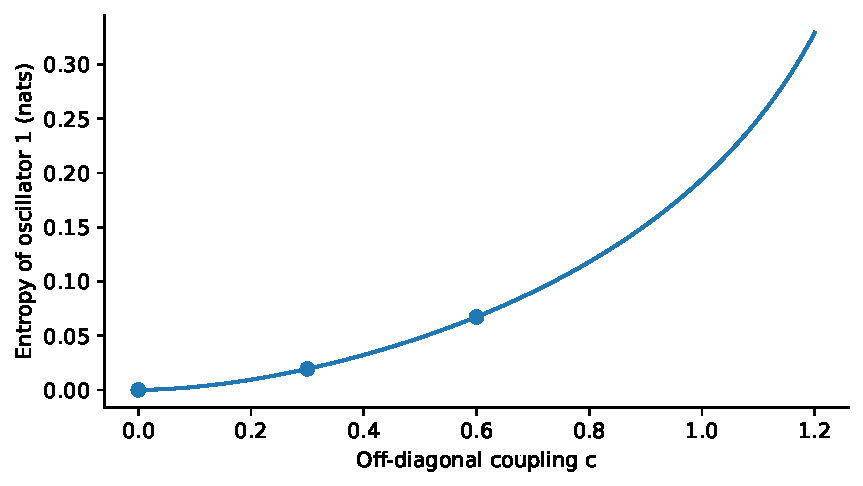
\includegraphics[width=.91\linewidth]{figures/oscillator_entropy.pdf}\caption{Entropy of one oscillator versus coupling. The marked points include the decoupled case and the two assigned benchmarks.}\end{figure}For real fields, $q_{-\bm{k}}=q_{\bm{k}}^\dagger$. A generic nonzero pair $\pm\bm{k}$ splits into two identical real cosine/sine sectors. Each contains one light and one spectator oscillator. We report $s(\nu_q)$ per real sector; the complete pair contributes $2s(\nu_q)$.\begin{thebibliography}{9}\small
\bibitem{gaussian} C. Weedbrook et al., \emph{Gaussian Quantum Information}, Rev. Mod. Phys. 84, 621 (2012), \href{https://arxiv.org/abs/1110.3234}{arXiv:1110.3234}.\end{thebibliography}
\textbf{Code and supporting data:} \href{https://github.com/rawatpriyansh17/QFT-PROJECT-GROUP-B/tree/main/step2}{step2 on GitHub}.\newpage\section*{Contributions (equal)}\begin{center}\begin{tabularx}{\linewidth}{p{33mm}X}\toprule Member & Contribution\\\midrule Priyansh Rawat & Normal-mode derivation and benchmark review.\\[3mm]Samarth Bhatnagar & Reduced-state covariance and rescaling checks.\\[3mm]Mayank Sinha & Numerical diagonalisation, purity cross-check and figure.\\\bottomrule\end{tabularx}\end{center}\end{document}